\section{Problem Statement and Motivation}
Incentives are powerful tools long employed to encourage certain behaviours. In the context of a business, several implementation options are available, such as posters, emails, websites, employee workshops, and campaigns; but another commonly adopted method is that of a loyalty scheme. Loyalty applications available range from the basic stamp/sticker book, to the more modern smartcards (Fig.~\ref{fig:smartcard}).

Commonly, simple paper-based systems are adopted by businesses due to low cost and implementation times; nonetheless systems like these have several issues
\begin{enumerate}
\item Some individuals may lose their stamp cards
\item There is an environmental impact associated with constantly printing stamp cards
\item Paper-based systems are not very secure and open to abuse
\end{enumerate}

An opportunity exists for a general-purpose system to encompass loyalty programs via use of up-and-coming Near-Field Communication (NFC) technologies that are integrated inside modern smart phones. Moreover, elements of `gamification' can be added as an extra dimension of loyalty to corporate persuasive technologies. (e.g. unlocking badges as they claim rewards, essentially playing versus themselves)

\begin{figure}[h!]
    \centering
    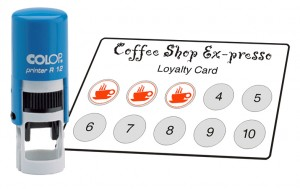
\includegraphics[width=0.5\textwidth]{img/Loyalty-card.jpg}
    \qquad
    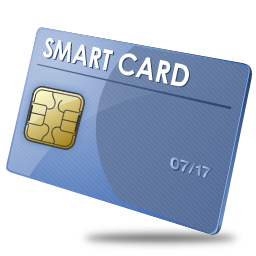
\includegraphics[width=0.3\textwidth]{img/smartcard.png}
    \caption{A paper stamp card \& smart card}%
    \label{fig:smartcard}
\end{figure}
\clearpage{}

\section{Rationale}
The smartphone is now a staple item which many people cannot leave their home without. As of 2014, there is a worldwide user-base of approximately 1.75 billion smartphone devices~\cite{smartUsers}. Migration to phones allow the business to have a central hub of all of their loyalty schemes, eradicating the need for paper. This means that issues relating to paper-based systems, such as printing paper (environmental impact) and people losing their stampcards are no longer an issue. Moreover, businesses will now have the option to track use and monitor their schemes for further analysis. This grants them insight into how many users they have, allowing them to adjust loyalty schemes appropriately.

On the other hand the proposed solution is not without some problems of its own. For instance, not everybody owns a smartphone, so hybrid smartphone/paper solutions will need to be considered. Additionally, there exists specific disadvantages of smartphones, such as dependence on battery life and an internet connection.

\section{Aim}
The aim of this project is to develop a general purpose solution using a smartphone that supports businesses in creating, managing and deploying a simple loyalty scheme - using gamification elements to engage the users. The specific technology chosen is NFC in phones running the Android operating system. 

\section{Objectives}
\begin{itemize}
    \item Research the state-of-art surrounding NFC technology within loyalty and gamification systems
    \item Examine and analyse the current smartphone solutions available to manage loyalty systems
    \item Design and implement our solution
    \item Perform a field study with the system as an evaluation
    \item Look into the future possibilities of the system and the infrastructural requirements to support its use in a real-world environment
\end{itemize}

\section{Deliverables}
The primary deliverables we perceive for this project are two Android applications. A `Loyalty Stampbook' application for consumers to collect, manage and use their loyalty schemes -- along with a `Loyalty Manager' for businesses/employees to distribute `stamps' to customers via NFC.  

\section{Significance \& Contributions}
NFC is a topic rising in popularity. Many new mobile smartphones now have a chip for NFC communication and many businesses are moving their `card' based services onto smartphones. As such, it is beneficial to explore the possibilities of transferring traditional loyalty cards into the digital era. 

Our solution provides a unique paper-less way for businesses to disseminate a loyalty scheme. We attempt to alleviate much of the hassle and cost to businesses with regards to implement

Moreover, we aimed to keep the solution very generic as to allow an element of branding and customisability, as well as using open protocols to extend the system to other mobile operating systems.   

\subsection{Similar Developments}
There exist some similar mobile-based solutions to the one proposed, such as Apple's \emph{PassBook}. Passbook is an iOS exclusive application that allows users to save their generic cards (i.e. boarding passes, event tickets, loyalty cards etc.) Though also a general purpose solution, there is a distinction on the technologies used (QR/Barcode Scanning) and the interactions presented to the users - For example, Passbook entails the one-way interaction of simply scanning barcodes. By adopting the two-way possibilities provided by NFC, richer interactions can be built and allow inter-communication between devices. Section \ref{sec:NFCvsQR} will discuss the advantages and disadvantages of each technology.

Other loyalty applications also exist, some using some combination of NFC or gamification elements; nonetheless they are specific to their associated brand. Starbucks' application on iOS is one such example (Fig.~\ref{fig:starbucksios6}), offering users a digital QR version of their Starbucks card (Fig.~\ref{fig:starbucksios6}c) and a medium to collect rewards in the form of stars. These stars, along with the account balance can be used to claim rewards and beverages. The opportunity of our proposed solution is to make an encompassing general-purpose solution that any business, big or small, can use to simply implement a loyalty program.

\begin{figure}[h!]
  \centering
    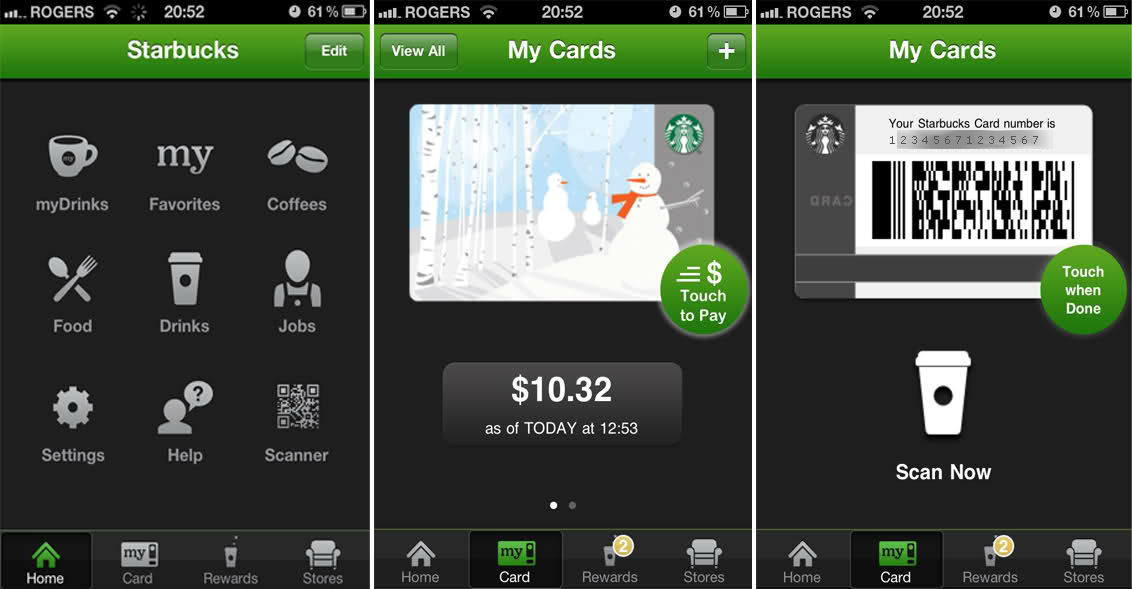
\includegraphics[width=1\textwidth]{img/starbucks-image-2.jpeg}
      \caption{Starbucks application for iOS6 (a) The menu of the Starbucks app (b) The card and available balance (c) The bar-code presented to the baristas to scan}
      \label{fig:starbucksios6}
\end{figure}

In the literature survey we shall cover primary technologies and research that enable these developments, along with confirming the need for a general-purpose solution.

\section{Resources Required}
\subsection{Technologies}
\subsubsection{Android Platform}
Android is a smartphone operating system developed by Google. Along with Windows Mobile OS and Apple's iOS, these three operating systems are the biggest players in the global smartphone market. Android was selected for our system was most devices are equipped with an NFC chip and have well supported APIs regarding Host Card Emulation (See \ref{sec:initalHCE}). With the introduction of iOS8, Apple now has support for NFC payments that work with the new iPhone 6; however APIs are unavailable to developers at this time and as a result, cannot be used. Windows Phone has similar NFC libraries to Android, but was not chosen due to it's low market share (2.5\% as a pose to Android's 84.7\%)\cite{marketShare}. 
\subsubsection{Android SDK}
The Android Software Development Kit (SDK) Will be required to develop, implement and test the Android applications. There are several methods that can be chosen regarding Android application development without having to use Google's JAVA SDK. Unfortunately, due to the specific dependencies on Google's NFC APIs, development will need to be done using the JAVA SDK.
\subsubsection{Host Card Emulation (HCE)}
\label{sec:initalHCE}
NFC chips can be placed into Card Emulation mode in such a way (ISO 14443) that a reader classifies it in the same manner as a smartcard.\cite{ecosystem}. Implementation of the system is dependent on use of this NFC facet. \emph{Android 4.4 Kitkat} and above support this mode within the APIs.
\subsection{Android Devices}
For most cases of Android development, the bundled emulator with Google's Android SDK is sufficient; however due to the project's dependence on the NFC chip, at least two physical (preferably differently branded) devices need to be used. One will be running the Loyalty Manager, whilst others will be running our Loyalty Stampbook. Both devices must at least have the \emph{Kitkat 4.4} iteration of Android in order to use Host Card Emulation.

\section{Dissertation Overview}
The rest of the dissertation is presented in the following chapters:
\begin{description}[leftmargin=!,labelwidth=\widthof{\bfseries Medium}]
    \item[Chapter 2] \emph{Literature \& Technical Survey} -- Here we will introduce the research topics of `NFC', `gamification' and `persuasive technologies' and review their applications to the world of mobile applications. 
    \item[Chapter 3] \emph{Requirements \& Design} -- Divulges the process of outlining the design of the system.
    \item[Chapter 4] \emph{Implementation} -- A detail account of the system was built, along with the novel challenges presented. 
    \item[Chapter 5] \emph{Evaluation} -- A field study with users in a natural environment. We attempt to gather quantitative and qualitative feedback, whilst trying to quantify the impact of gamification within the system. 
    \item[Chapter 6] \emph{Discussion}
    \item[Chapter 7] \emph{Conclusions \& Future Work} -- A closing discussion for our system and the vision for the future. 
\end{description}